\documentclass[11pt]{article}
\usepackage[T1]{fontenc}
\usepackage{lmodern}
\usepackage[margin=1in]{geometry}
\usepackage{amsmath,amssymb,amsthm}
\usepackage{booktabs}
\usepackage{microtype}
\usepackage{tikz}
\usepackage[colorlinks=true,linkcolor=blue,citecolor=blue,urlcolor=blue]{hyperref}
\hypersetup{pdftitle={Greedy play can require more colors in the coloring game},pdfauthor={P. Graham}}
\newtheorem{theorem}{Theorem}
\newtheorem{lemma}{Lemma}
\newcommand{\chig}{\chi_g}
\newcommand{\Gammag}{\Gamma_g}
\newcommand{\N}{\mathbb{N}}
\title{Greedy play can require more colors in the coloring game}
\author{P. Graham\\ \small\url{https://orcid.org/0009-0007-8493-1505}}
\date{October 26, 2026}

\begin{document}
\maketitle
\begin{abstract}
In the coloring game, Alice and Bob alternately color vertices properly
from a fixed palette, with Alice trying to color the whole graph.
The game chromatic number is the least palette size for which she can win.
In the greedy game the players choose vertices, each receiving the least
available positive integer; Alice minimizes and Bob maximizes the number
of colors used. Havet and Zhu asked in June 2011 whether the resulting
game Grundy number is always at most the game chromatic number.
We give an explicit finite simple graph $G$ for which
$\chig(G)=5$ and $\Gammag(G)=6$, answering the first part of their question
negatively. The proof consists of finite strategy certificates checked by two separately written
certificate checkers for the two unrestricted Alice-first games, together with
a clique obstruction and a short greedy strategy. It does not
establish arbitrarily large separation between the parameters.

This work has not yet been reviewed by experts.
The proofs, the search code, the certificate checkers and the text were
produced by AI models (from OpenAI and Anthropic), working under the
author's direction.
\end{abstract}

\noindent Computer-assisted. 

\smallskip
\noindent 
An outside AI model suggested the clique and degree observations used for the exact values.

\section{Introduction}
The ordinary coloring game is played on a finite simple graph with a
palette of $k$ colors. Alice and Bob alternately give an uncolored vertex
a color different from those of its colored neighbors. Alice wins if the
whole graph is colored; otherwise Bob wins. The least $k$ for which Alice
has a winning strategy is the \emph{game chromatic number} $\chig(G)$.
In the greedy game, a chosen vertex receives the least positive integer
absent from its colored neighbors. Alice minimizes and Bob maximizes the
largest color used. The value is the \emph{game Grundy number} $\Gammag(G)$.
Alice moves first in both games, either player may choose any uncolored
vertex, and neither player may pass.

\begin{theorem}\label{thm:main}
The graph $G$ defined in Section~\ref{sec:graph} is a finite simple graph
with $11$ vertices and $27$ edges satisfying
\[
             \chig(G)=5, \qquad \Gammag(G)=6.
\]
Both values concern unrestricted vertex selection with Alice
moving first, alternating turns, and no passes.
\end{theorem}

Havet and Zhu introduced the game Grundy number in a report first posted
on June 15, 2011. The first sentence of Problem~5 in version~1 reads:
\begin{quote}
``Is it true that $\Gamma_g(G)\leq\chi_g(G)$ for all graph $G$?''
\end{quote}
The problem then asks separately whether the game Grundy number can be
arbitrarily large compared with the game chromatic number~\cite[p.~6]{HZ}.
Theorem~\ref{thm:main} answers the first part negatively. It does not
answer the second part, and makes no assertion about the smallest
possible counterexample.

Hollom restated the inequality as Question~3.4 and explained an obstacle
to transferring an ordinary winning strategy to greedy
play~\cite{Hollom}. Hollom's ordered-game example concerns a prescribed
sequence of vertex locations. It does not itself give an unrestricted
counterexample. The new contribution here is an explicit graph together
with an ordinary winning strategy for Alice and a greedy strategy for Bob
that survives every legal choice of vertex by Alice. This universal
coverage of Alice's choices is the essential additional obligation beyond
an ordered example; it is supplied by the finite certificates.

There is also a distinct question in the reverse direction. Krawczyk
and Walczak proved that the game chromatic number is not bounded by a
function of the ordinary, static Grundy number~\cite[Theorem~7]{KW}.
The static Grundy number is the maximum number of colors used by greedy
coloring over all vertex orders, so it is at least $\Gammag(G)$.
Their theorem therefore also rules out bounding $\chig(G)$ by a function
of $\Gammag(G)$. This earlier result concerns the reverse boundedness
question, rather than the inequality answered here. The present proof
uses the definitions and question of Havet and Zhu and the distinction
emphasized by Hollom; it does not use the construction of Krawczyk and
Walczak.

Nearby work studies connected greedy coloring (Lima, Marcilon, Martins
and Sampaio~\cite{LMMS}; Marcilon and Ribeiro~\cite{MR}), ordinary coloring
on complete multipartite graphs (Furtado, Dantas, de Figueiredo and
Del-Rio-Palma~\cite{FDDP}), majority coloring games (Chawda, Nanoti,
Sankarnarayanan and Srinivasan~\cite{CNSS}), connected games on corona
products (Mesari\v{c} \v{S}tesl~\cite{MS}), and the difference from the ordinary
chromatic number (Hollom~\cite{HollomGap}). Costa, Pessoa, Sampaio and
Soares~\cite{CPSS} and Marcilon, Martins and Sampaio~\cite{MMS} study
computational complexity; Figueiredo and dos Santos~\cite{FS} study
two-turn asymmetric games. Nothing from these nearby works is used here.

Section~\ref{sec:overview} describes the proof and the finite games used
in the certificates. Section~\ref{sec:graph} specifies the graph.
Section~\ref{sec:proof} gives the certificate argument, and
Section~\ref{sec:checking} describes the reproducible checks.

\section{Games and proof overview}\label{sec:overview}
The proof compares two games on the same graph with the same five
colors; it does not compare separate graph families or rely on changing
the palette of an ordinary strategy.

For example, if a vertex has colored neighbors using color $1$ and no
other color, an ordinary move with five colors may give it any of
$2,3,4,5$. The greedy move must give it color $2$. Although greedy moves
form a subset of ordinary moves at a fixed position, both players are
subject to this restriction. An ordinary winning strategy for Alice may
ask her to make a move that the greedy rule forbids.

Write $V(G)$ for the vertex set and $N_G(v)$ for the neighbors of a vertex
$v$. A palette-$k$ position is a function
\[
       s:V(G)\longrightarrow\{0,1,\ldots,k\},
\]
where $0$ denotes an uncolored vertex and adjacent nonzero values must
differ. For an uncolored vertex $v$, define its available colors by
\[
 A_k(s,v)=\{1,\ldots,k\}\setminus
              \{s(u):u\in N_G(v),\ s(u)\ne0\}.
\]
An ordinary legal move chooses any uncolored $v$ and any
$c\in A_k(s,v)$. A greedy legal move in the palette-$k$ game chooses
any uncolored $v$ with $A_k(s,v)\ne\varnothing$ and uses
$c=\min A_k(s,v)$. In each case the new position changes only $s(v)$,
from $0$ to $c$.

The certificates stop a palette-$k$ game as soon as either all vertices
are colored, an Alice win, or an uncolored vertex has no available color,
a Bob win. Such a vertex is called \emph{blocked}. An ordinary game may
instead be described as continuing until no legal move remains. These
conventions have the same winner: once a vertex is blocked, its neighbors'
colors never disappear, and a full coloring is impossible.

The unrestricted greedy game has no fixed palette. A selected vertex
always receives the least positive integer absent from its colored
neighbors, so a move is possible until every vertex is colored. Its used
colors form an initial interval of the positive integers: a first use
of color $c$ requires colored neighbors of every smaller positive color.
Consequently its largest color and its number of colors agree.

The two original certificates give the outer bounds. The ordinary certificate selects a legal move
for Alice and covers every legal move by Bob. It forces a full proper
coloring from the five-color palette. The greedy certificate selects a
legal move for Bob and covers every greedy move by Alice. It forces a
blocked vertex in the palette-five game. Since the five colors on that
vertex's neighbors persist, unrestricted greedy play must eventually
use a color at least six. A five-vertex clique supplies the matching
ordinary lower bound. For the greedy upper bound, Alice ensures that the
only two vertices of degree greater than five are colored within the
first three moves.
Every other vertex then receives a color at most six.

Each certificate is a directed graph of literal labeled positions.
Different histories reaching the same position share its continuation.
There is no quotient by graph automorphisms or by color permutations.
Every arc colors one additional vertex, so correctness reduces to a
finite induction. The argument establishes two specific strategies; it
requires neither a search over all graphs nor an exhaustive solution of
every position in either game.

\section{The graph}\label{sec:graph}
The following list specifies the example independently of its drawing.
Its vertices are $0,1,\ldots,10$. In the right column of
Table~\ref{tab:edges}, each entry $v$ in row $u$ denotes the edge
$\{u,v\}$; only neighbors with larger labels are listed. Thus each edge
appears exactly once, and there are no additional edges.

\begin{table}[ht]
\centering
\begin{tabular}{r@{\qquad}l r@{\qquad}l}
\toprule
$u$ & Neighbors greater than $u$ & $u$ & Neighbors greater than $u$\\
\midrule
0 & $3,5,7,8$       & 6 & $9,10$\\
1 & $4,6,8,9,10$    & 7 & $9$\\
2 & $5,6,7,9,10$    & 8 & $10$\\
3 & $7$            & 9 & $10$\\
4 & $6,8,9,10$     &10 & $\varnothing$\\
5 & $7,8,10$       &   & \\
\bottomrule
\end{tabular}
\caption{The complete edge list of $G$, grouped by smaller endpoint.}
\label{tab:edges}
\end{table}

\begin{figure}[ht]
\centering
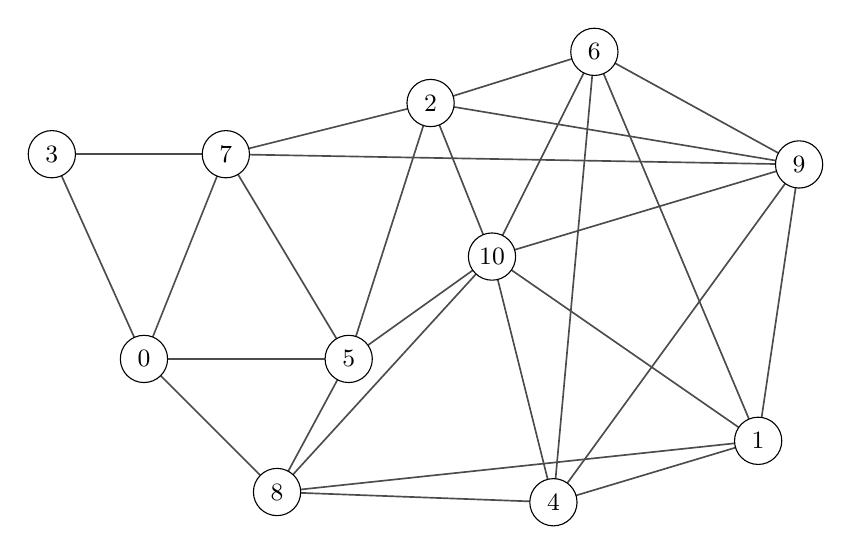
\begin{tikzpicture}[x=1.3cm,y=1.3cm,
  vertex/.style={circle,draw,fill=white,minimum size=6mm,inner sep=0pt,font=\small}]
  \coordinate (v0) at (0.7,2.0);
  \coordinate (v1) at (6.7,1.2);
  \coordinate (v2) at (3.5,4.5);
  \coordinate (v3) at (-0.2,4.0);
  \coordinate (v4) at (4.7,0.6);
  \coordinate (v5) at (2.7,2.0);
  \coordinate (v6) at (5.1,5.0);
  \coordinate (v7) at (1.5,4.0);
  \coordinate (v8) at (2.0,0.7);
  \coordinate (v9) at (7.1,3.9);
  \coordinate (v10) at (4.1,3.0);
  \begin{scope}[draw=black!70,line width=0.6pt]
    \draw (v0) -- (v3);
    \draw (v0) -- (v5);
    \draw (v0) -- (v7);
    \draw (v0) -- (v8);
    \draw (v1) -- (v4);
    \draw (v1) -- (v6);
    \draw (v1) -- (v8);
    \draw (v1) -- (v9);
    \draw (v1) -- (v10);
    \draw (v2) -- (v5);
    \draw (v2) -- (v6);
    \draw (v2) -- (v7);
    \draw (v2) -- (v9);
    \draw (v2) -- (v10);
    \draw (v3) -- (v7);
    \draw (v4) -- (v6);
    \draw (v4) -- (v8);
    \draw (v4) -- (v9);
    \draw (v4) -- (v10);
    \draw (v5) -- (v7);
    \draw (v5) -- (v8);
    \draw (v5) -- (v10);
    \draw (v6) -- (v9);
    \draw (v6) -- (v10);
    \draw (v7) -- (v9);
    \draw (v8) -- (v10);
    \draw (v9) -- (v10);
  \end{scope}
  \node[vertex] at (v0) {0};
  \node[vertex] at (v1) {1};
  \node[vertex] at (v2) {2};
  \node[vertex] at (v3) {3};
  \node[vertex] at (v4) {4};
  \node[vertex] at (v5) {5};
  \node[vertex] at (v6) {6};
  \node[vertex] at (v7) {7};
  \node[vertex] at (v8) {8};
  \node[vertex] at (v9) {9};
  \node[vertex] at (v10) {10};
\end{tikzpicture}

\caption{The graph $G$. Crossings in the drawing are not vertices.
The drawing is generated from the edge list in \texttt{data/graph.json}.}
\label{fig:graph}
\end{figure}

The machine-readable graph is \texttt{data/graph.json}. All three strategy
certificates contain the same vertex set and edge list, and the public
entry point checks their equality to this graph before checking either
strategy. It binds the original pair to palette size five and the new
greedy certificate to palette size six, all with Alice-first play and
unrestricted vertex selection. The ordinary
certificate's first move colors vertex $5$ with color $1$; subsequent
choices are given by its positions and arcs, rather than by a short
case-based strategy in the text.

\section{Why the certificates prove the theorem}\label{sec:proof}
This section gives the finite induction behind the checks and explains
why the greedy certificate implies a lower bound in the unrestricted
game.

\subsection{Local strategy obligations}
A strategy certificate declares a game, a starting player, a palette
size, a graph and a claimed winner. Its nodes are proper partial
colorings. The root is the all-zero position. A node lists moves
$(v,c)$, each leading to the position obtained by assigning color $c$
to the previously uncolored vertex $v$. Alice moves when the number of
colored vertices is even; Bob moves when it is odd.

At every reachable node the checker recomputes all legal moves directly
from the graph and the partial coloring. A terminal node lists no moves,
and its recomputed winner must be the declared winner. At a nonterminal
node belonging to the declared winner, the certificate lists exactly
one legal move. At a nonterminal node belonging to the other player,
it lists exactly all legal moves, without duplication. Every listed
successor must be present, and all nodes must be reachable from the root.

\begin{lemma}\label{lem:strategy}
Consider either palette-$k$ game defined in
Section~\ref{sec:overview}, with Alice first and with stopping at a
blocked vertex. If a finite certificate satisfies the local strategy
obligations above, its declared winner has a winning strategy from the
all-zero position.
\end{lemma}

\begin{proof}
For each certificate position $s$, induct on the number of its uncolored
vertices. A terminal position has the declared winner by the terminal
check. At a nonterminal position where that winner moves, the selected
legal move leads to a position with one fewer uncolored vertex, which
is winning by induction. At a position where the opponent moves, all
legal moves are included, and every successor is winning by induction.
This proves the claim at every reachable position, including the root.
The strict increase in the number of colored vertices along each arc
also rules out cycles.
\end{proof}

\subsection{From a blocked vertex to a sixth greedy color}
The lower bound uses a threshold certificate, so its connection with the
unrestricted greedy game needs a separate argument.

\begin{lemma}\label{lem:bridge}
Let $H$ be a finite simple graph. Suppose Bob has a winning strategy in
the Alice-first greedy palette-$k$ game of
Section~\ref{sec:overview}, with unrestricted vertex selection,
alternating turns, no passes, and stopping when a vertex is blocked.
Then Bob can force a color greater than $k$ in the unrestricted greedy
game on $H$. In particular, $\Gammag(H)>k$.
\end{lemma}

\begin{proof}
Until a blocked vertex occurs, every uncolored vertex has some available
color in $\{1,\ldots,k\}$. Its least available positive integer is
therefore the same in the unrestricted game and in the palette-$k$
game. Bob follows his palette-$k$ strategy during this common part of
play. Every choice of vertex by Alice is a legal choice in the threshold
game and is covered by that strategy.

Bob's winning strategy reaches a blocked vertex $v$ before a full
coloring. At that point every color in $\{1,\ldots,k\}$ occurs on a
colored neighbor of $v$. These colors persist. The unrestricted game
continues until all vertices are colored, since each turn colors one
previously uncolored vertex and no player may pass. When $v$ is colored,
its greedy color is consequently greater than $k$. Thus Bob forces
the required lower bound, regardless of subsequent moves.
\end{proof}

\subsection{The matching local bounds}
The remaining bounds use only the labeled graph and a short opening strategy.

\begin{lemma}\label{lem:local}
The graph $G$ satisfies $\chig(G)\geq5$ and $\Gammag(G)\leq6$.
\end{lemma}

\begin{proof}
All ten pairs of vertices in $\{1,4,6,9,10\}$ are edges in
Table~\ref{tab:edges}. Every complete proper coloring therefore uses
at least five colors, so Alice cannot win with any smaller palette.

Every vertex outside $\{9,10\}$ has degree at most five. A vertex of
degree $d$ receives a greedy color at most $d+1$: a larger color would
require distinct colored neighbors of every smaller positive color.
Alice first chooses vertex $10$, which receives color $1$.
If Bob chooses vertex $9$ on move two, its color is at most $2$.
Otherwise Alice chooses $9$ on move three, when its color is at most
$3$ because only two vertices have been colored. In either branch,
both exceptional vertices are colored by move three. All later choices
are among vertices of degree at most five and receive colors at most
six. Alice may choose any remaining vertex thereafter. Each move
colors a new vertex, so play finishes after eleven moves, with at most
six distinct colors, for every legal Bob response.
\end{proof}

\begin{proof}[Proof of Theorem~\ref{thm:main}]
Table~\ref{tab:edges} specifies a simple graph of the stated order and
size. The two checks described in Section~\ref{sec:checking} accept an
ordinary certificate with declared winner Alice and a greedy
certificate with palette $k=5$ and declared winner Bob for this graph and
the stated conventions.

By Lemma~\ref{lem:strategy}, Alice has a winning ordinary strategy with
five colors. Hence $\chig(G)\leq5$ directly from the definition as the
least winning palette size. No assertion that ordinary winning
palettes are monotone is needed. The same lemma gives Bob a winning
strategy in the greedy palette-five game. Lemma~\ref{lem:bridge} then
gives $\Gammag(G)>5$. Combining these outer bounds with
Lemma~\ref{lem:local} proves the two exact values.
\end{proof}

\section{Finite verification and reproducibility}\label{sec:checking}
The bundle contains the graph, the three finite strategies and two
separately written certificate checkers. Checking requires Python 3
and its standard library, with no graph generator, search executable
or external mathematical package. From the bundle's top-level directory,
the command is
\begin{verbatim}
python3 -I checks/verify.py
\end{verbatim}
The same command checks all three certificates, the local graph facts,
and the corruption tests. Detailed format and checker documentation is in
\texttt{checks/README.md}.

\subsection{Data and checker independence}
The files \texttt{data/ordinary-k5.json.gz},
\texttt{data/greedy-k5.json.gz} and \texttt{data/greedy-k6.json.gz}
are gzip-compressed JSON objects.
Besides the game conventions and graph, each contains a map from
comma-separated color vectors to lists of moves. The coordinate order
is the vertex order $0,\ldots,10$; $0$ is the uncolored marker.
All states and moves are labeled literally. A strategy can discard
unneeded choices at its winner's turns, while retaining every legal
choice at the opponent's turns. The resulting sizes are reported in
Table~\ref{tab:certificates}; these are certificate sizes, not full
game-tree sizes.

\begin{table}[ht]
\centering
\begin{tabular}{llrrr}
\toprule
Game & Declared winner & Nodes & Arcs & Terminal nodes\\
\midrule
Ordinary, $k=5$ & Alice & $108\,669$ & $216\,995$ & $2\,800$\\
Greedy, $k=5$ & Bob & $5\,594$ & $6\,730$ & $2\,010$\\
Greedy, $k=6$ & Alice & $2\,223$ & $3\,339$ & $208$\\
\bottomrule
\end{tabular}
\caption{The finite strategy certificates.}
\label{tab:certificates}
\end{table}

The programs \texttt{checks/check.py} and
\texttt{checks/check\_independent.py} implement the local obligations
of Section~\ref{sec:proof} separately. Neither imports the search
program or the other checker. They reconstruct adjacency, properness,
available colors, the player to move, legal moves and terminal outcomes
from each certificate. In particular, terminal winners are recomputed;
they are not trusted labels attached to leaves. The entry point also
checks the graph and game bindings against the public statement's
five-color outer bounds and six-color upper bound. Thus acceptance of a different graph, a
different starting player or an ordered variant cannot substitute for
the game obligations used in the theorem.

\subsection{Corruption tests and trusted components}
For each original five-color certificate the public command makes seven semantic changes:
it omits an opponent reply, reverses the declared winner, inserts an
illegal Alice move, adds an edge, changes the starting player, treats
the root as a terminal node, and adds a move at a terminal node.
Each altered certificate is submitted directly to both checkers, and
both must reject it. The command therefore requires $28$ rejection
outcomes in addition to accepting the two unchanged certificates.
These controls exercise game semantics rather than file-integrity checks.

The six-color Alice certificate follows the opening in Lemma~\ref{lem:local}
and then selects the smallest uncolored label on Alice's turns. Every Bob
reply is retained. All its leaves are full colorings, so no early threshold
stop replaces unrestricted greedy completion. Both checkers reject eight
changes: a missing Bob reply, an Alice pass, a nonleast greedy color,
ordered play, Bob moving first, an unfinished leaf, threshold five, and a
missing successor. The local-fact check also rejects a deleted clique edge,
a violation of the degree bound, and a cyclic shift of the vertex labels.

The proof relies on the correctness of the two Python implementations,
the Python interpreter and its JSON and gzip libraries, and the written
finite-induction and blocked-vertex arguments above. The certificate
checks use exact integer and finite-set operations. The graph drawing
is generated from the graph data, and its edges are checked against
that data; the mathematical definition of $G$ remains the edge list.
The checks in this bundle run in Python. The search that found the
graph is unnecessary for checking the theorem, and no exhaustive graph
search or claim of minimality is part of the result.

\begin{thebibliography}{99}

\bibitem{HZ}
Fr\'ed\'eric Havet and Xuding Zhu,
\emph{The game Grundy number of graphs},
Research Report RR-7646, INRIA, version~1, first posted June 15, 2011.
Problem~5, p.~6.
\url{https://inria.hal.science/inria-00600738v1/document}.

\bibitem{Hollom}
Lawrence Hollom,
\emph{On monotonicity in Maker-Breaker graph colouring games},
arXiv:2308.03528, version~2.
First posted August 7, 2023; revised November 8, 2024.
Question~3.4.
\url{https://arxiv.org/abs/2308.03528v2}.

\bibitem{KW}
Tomasz Krawczyk and Bartosz Walczak,
\emph{Asymmetric coloring games on incomparability graphs},
arXiv:1503.04748, first posted March 16, 2015.
Theorem~7.
\url{https://arxiv.org/abs/1503.04748}.


\bibitem{LMMS}
Carlos V. G. C. Lima, Thiago Marcilon, Nicolas Martins and Rudini Sampaio,
\emph{The connected greedy coloring game},
Theoretical Computer Science 940 (2023), 1--13; online October 26, 2022.
\url{https://doi.org/10.1016/j.tcs.2022.10.034}.

\bibitem{MR}
Thiago Marcilon and Ariane Ribeiro,
\emph{Results on the connected greedy coloring game},
LAWCG 2024 annals, p.~48, October 20--23, 2024;
journal version, Matem\'atica Contempor\^anea 62 (2026), 25--32,
online September 23, 2025.
\url{https://www.lawcg.mat.br/lawcg24/LAWCG2024-annals.pdf}.
\url{https://doi.org/10.1007/s44425-025-00018-3}.

\bibitem{FDDP}
Ana Lu\'isa C. Furtado, Simone Dantas, Celina M. H. de Figueiredo and
Miguel Del-Rio-Palma,
\emph{Coloring game on complete multipartite with singletons and equal sized parts},
Discrete Mathematics 349 (2026), 115291; online June 23, 2026.
\url{https://doi.org/10.1016/j.disc.2026.115291}.

\bibitem{CNSS}
Yash Chawda, Saraswati Girish Nanoti, Brahadeesh Sankarnarayanan and
Eshwar Srinivasan,
\emph{Structural and computational aspects of majority coloring games},
arXiv:2609.37796, first posted September 29, 2026.
\url{https://arxiv.org/abs/2609.37796}.

\bibitem{MS}
Da\v{s}a Mesari\v{c} \v{S}tesl,
\emph{Connected Coloring Games on Corona Products of Graphs},
arXiv:2610.29650, first posted October 21, 2026.
\url{https://arxiv.org/abs/2610.29650}.

\bibitem{HollomGap}
Lawrence Hollom,
\emph{On graphs with maximum difference between game chromatic number and chromatic number},
arXiv:2309.01583, first posted September 4, 2023; version~3, November 8, 2024.
Discrete Mathematics 348 (2025), 114271; online September 26, 2024.
\url{https://arxiv.org/abs/2309.01583v3}.

\bibitem{CPSS}
Eurinardo Rodrigues Costa, Victor Lage Pessoa, Rudini Sampaio and Ronan Pardo Soares,
\emph{PSPACE-completeness of two graph coloring games},
Theoretical Computer Science 824--825 (2020), 36--45; online April 16, 2020.
\url{https://doi.org/10.1016/j.tcs.2020.03.022}.

\bibitem{MMS}
Thiago Marcilon, Nicolas Almeida Martins and Rudini Sampaio,
\emph{Hardness of some variants of the graph coloring game},
arXiv:1911.10363, first posted November 23, 2019.
\url{https://arxiv.org/abs/1911.10363}.

\bibitem{FS}
Eder Figueiredo and Vin\'icius Fernandes dos Santos,
\emph{Two-Turn Assymetric Graph Coloring Games},
Matem\'atica Contempor\^anea \textbf{62} (2026), 86--93; online September 26, 2025.
\url{https://doi.org/10.1007/s44425-025-00025-4}.

\end{thebibliography}
\end{document}
